\scanpage{96}

trois, compatibles avec un $\overline{\mathrm m}$ hom
\diagram{\begin{tikzcd}[ampersand replacement=\&,column sep=large]
\mathcal M_{\deleted{\unsure{0}}} \arrow[r] \&
\deleted{\unsure{\mathbb O|\Phi}}\gamma_{\rho,\sigma}
\overset{\unsure{\mathrm{def}}}{=}
\underbrace{\unsure{\underline{\gamma}_{\rho,\sigma}^{*}|\underline{\gamma}_{\rho,\sigma}^{\bullet}}}_{\mathbb O_{12}^{*}}
(\widehat{\mathbb Z})^{\Delta}
=\deleted{\unsure{\mathbb O_{12}^{*}}}\widehat{\mathbb Z}^{*}
\end{tikzcd}}
qui n'est autre que le caractère cyclotomique $\chi$.
\unsure{Un}\deleted{\unsure{le|de}} de ces trois,
\diagram{\begin{tikzcd}[ampersand replacement=\&,column sep=small,row sep=small]
\mathcal M \arrow[rr] \arrow[dr,dashed] \&\& N_{\rho}^{\sim}\arrow[r,"\sim"] \&\widehat{\mathbb Z}^{*},\\
\&\inserted{\Gamma_{\mathbb Q}^{\mathrm{et}}}\arrow[ur,dashed]\&\&
\end{tikzcd}}
se réduit ici \unsure{audit} caractère, et ne pose donc aucune question intéressante. On a d'autre part

\noindent (218)\quad
\diagram{\begin{tikzcd}[ampersand replacement=\&,column sep=large]
\mathcal M\arrow[r]\arrow[d]\&G_{\rho,\sigma}=\widehat{\mathbb Z}^{*}\mathbin{\cdot}\mathfrak S^{+\wedge}\arrow[d]\\
\mathcal M^{!}\arrow[r]\&G_{\rho,\sigma}^{\unsure{\natural|\sharp}}=\widehat{\mathbb Z}^{*}\mathbin{\cdot}M^{\wedge},
\end{tikzcd}}

qu'il faudra examiner de plus près --- comme le caractère cyclotomique est \inserted{($\overline{\mathrm m}$ sur $\mathcal M!$)} surjectif, on \unsure{sait} en tous cas que ces deux hom sont \uline{surjectifs}. Enfin, on a un hom
$\mathcal M\longrightarrow N_{\sigma}^{\unsure{\natural|\sharp}\deleted{\unsure{\mathrm{ab}}}}$, qui se factorise en

\noindent (219)\quad
\diagram{\begin{tikzcd}[ampersand replacement=\&,column sep=large]
\Gamma_{\mathbb Q}^{\mathrm{et}}\arrow[r]\&N_{\sigma}^{\unsure{\natural|\sharp}\deleted{\unsure{\mathrm{ab}}}}=\widehat{\mathbb Z}^{*}\mathbin{\cdot}\widehat{\mathbb Z}
\end{tikzcd}}
\hfill ($\frac12$ direct)

qu'il faudra examiner également --- notamment voir s'il est surjectif.
Bien entendu, je n'ai de chance de le faire que par ``voie arithmétique'', en \unsure{prouvant} que l'hom induit sur $\Gamma_{\mathbb Q}$ lui-même est épi.

\margin{95}

\scanpage{97}
\mspage{696}

J'ai envie de mettre ces homomorphismes en relation avec la ``tour'' des courbes algébriques définies sur $\mathbb Q$, indexées par $n\in\unsure{\mathbb N^{*}|\mathbb N^{\wedge}}$

\noindent (220)\quad
\diagram{\begin{tikzcd}[ampersand replacement=\&,column sep=small,row sep=small]
X_n : \arrow[d,phantom,"\subset" description,sloped] \& x_0^n+x_1^n+x_{\infty}^n=0\\
\mathbb P_{\mathbb Q}^{2}\&
\end{tikzcd}}
\hfill (courbe de Fermat d'indice $n$)

\inserted{Soit $U_n$ l'ouvert des pts où $x_0x_1x_{\infty}\ne0$}

Sur $X_n$ le schéma en groupes $\mu_n^{\{0,1,\infty\}}/\underbrace{\mu_n}_{\mathrm{diag}.}$ opère ($\mu_n={}_n\mathbb G_m$), \deleted{et \unsure{on a}} ainsi que $\mathfrak S_3=\mathfrak S_{\{0,1,\infty\}}$, donc aussi le produit semi-direct
\[
(221)\qquad \underline F_n=\mathfrak S_3\mathbin{\cdot}\underbrace{\mu_n^{\{0,1,\infty\}}/\mu_n}_{\underline F_n^{\circ}},
\]
\margin{\unsure{Notation} $F_n$ pas très \unsure{heureuse} --- il est possible qu'il y aura besoin pour la suite de la lettre $F_n$, $F_{\infty}$ pour les revêtements de Fermat $U_n$, $U_{\infty}$ eux-mêmes\unsure{\ldots} (comparer \unsure{rectificatifs|rectifications} p.~719!)}
on a
\[
(222)\qquad X_n/\underline F_n^{\circ}\simeq X_1\simeq U_{0,3},
\]
l'isomorphisme compatible avec les actions de $\mathfrak S_3$. Plus généralement, on a, si $n=n'd$, un hom

\noindent (223)\quad
\diagram{\begin{tikzcd}[ampersand replacement=\&,column sep=large,row sep=small]
X_{\unsure{n=n'd}}\arrow[r,very thick]\&X_{n'}\\
x_i\arrow[r,mapsto]\&x_i^d
\end{tikzcd}}

et de cette façon $\deleted{X_n}\inserted{U_n}$ devient un revêtement principal (= torseur) sur $\deleted{X_{n'}}\inserted{U_{n'}}$, de groupe $\mu_d^{\{0,1,\infty\}}/\mu_d$, De façon plus précise encore, \deleted{(223) est compatible avec}

\noindent \deleted{(224)}\quad
\diagram{\begin{tikzcd}[ampersand replacement=\&,column sep=large,row sep=small]
\deleted{F_n}\arrow[r,"\deleted{\text{épi}}","\deleted{\unsure{\text{canonique}}}"']\arrow[d,equal]\&\deleted{F_{n'}}\arrow[d,equal]\\
\deleted{\mathfrak S_3\mathbin{\cdot}\mu_n^{\{0,1,\infty\}}}\&\deleted{\mathfrak S_3\mathbin{\cdot}\mu_{n'}^{\{0,1,\infty\}}}
\end{tikzcd}}
\deleted{$\left\{\begin{aligned}g&\longmapsto g\quad\text{si }g\in\mathfrak S_3,\\(x_0,x_1,x_{\infty})&\longmapsto (x_0^d,x_1^d,\unsure{x_{\infty}^d})\end{aligned}\right.$}

\margin{96}

\scanpage{98}

\deleted{et $\mu_n^{\{0,1,\infty\}}$, à fortiori $\mu_d^{\{0,1,\infty\}}$, opère librement sur $X_n$, et on trouve par passage au quotient} \unsure{on a} une suite exacte can.

\noindent (224)\quad
\diagram{\begin{tikzcd}[ampersand replacement=\&,column sep=small,row sep=small]
1\arrow[r,no head]\&\mu_d^{\{0,1,\infty\}}\deleted{/\mu_d}\arrow[r]\&
\begin{gathered}\underline F_n\\ \Vert\\ \unsure{\mathfrak S_{3\,S_0}}\mathbin{\cdot}\mu_n^{\{0,1,\infty\}}\end{gathered}\arrow[r]\&
\begin{gathered}\underline F_{n'}\\ \Vert\\ \mathfrak S_{3\,S_0}\mathbin{\cdot}\mu_{n'}^{\{0,1,\infty\}}\end{gathered}\arrow[r]\&1\\
\&(x_0,x_1,x_{\infty})\arrow[r,mapsto]\&(x_0,x_1,x_{\infty})\&\&\\
\&\&(x_0,x_1,x_{\infty})\arrow[r,mapsto]\&(x_0^d,x_1^d,x_{\infty}^d)\&\\
\&\&g\deleted{\unsure{\in\mathfrak S_3}}\arrow[r,mapsto]\&g\&
\end{tikzcd}}
\[
\text{pour}\quad\begin{aligned}x_0,x_1,x_{\infty}&\in\Gamma\mu_n,\\g&\in\Gamma\mathfrak S_{3\,S_0}\end{aligned}\qquad\big)
\]

et \unsure{l'homomorphisme|l'isomorphisme} (223) est compatible avec (224), et induit un iso. (compatible avec actions de $F_{n'}$)
\[
(225)\qquad X_{n'}\simeq X_n/(\mu_d^{\{0,1,\infty\}}/\mu_d),
\]
De plus, l'action de $\deleted{\unsure{\mu_n^{\{0,}}}$
\[
\underline F_n^{\circ}=\mu_n^{\{0,1,\infty\}}/\mu_n
\]
sur $\inserted{U_n}\deleted{X_n}$ est libre, et à fortiori celle de $\mu_d^{\{0,1,\infty\}}/\mu_d$ l'est, de sorte que $\deleted{X_n}\inserted{U_n}$ est bien un torseur sur $\deleted{X_{n'}}\inserted{U_{n'}}$ de groupe
\[
\underline F_d^{\circ}=\mu_d^{\{0,1,\infty\}}/\mu_d
\]
Passant à la limite, on trouve
\[
(226)\qquad\left\{\begin{aligned}
X_{\infty}&=\varprojlim_{n\in\mathbb N^{*}}X_n,\quad U_{\infty}=\varprojlim U_n\\
\underline F_{\infty}&=\varprojlim\underline F_n=(\mathfrak S_3)_{S_0}\mathbin{\cdot}\deleted{\unsure{\widehat{\mathbb Z}^{2}}}\left(\widehat{\mathbb Z}^{\{0,1,\infty\}}/\widehat{\mathbb Z}\right)\otimes_{\widehat{\mathbb Z}}\unsure{T_{\bullet}(\mathbb G_m)|T(\mathbb G_m)}
\end{aligned}\right.
\]

\margin{97}

\scanpage{99}
\mspage{697}

avec opération de $F_\infty$ sur \deleted{$X_\infty$}\inserted{$U_\infty$}
\deleted{$F_\infty^\circ$ opère}
\[
(227)\qquad F_\infty^\circ=\varprojlim_n F_n^\circ\simeq
\inserted{\widehat{\mathbb Z}^{\{0,1,\infty\}}\otimes_{\widehat{\mathbb Z}}}
\unsure{T_\bullet|T_*}(\mathbb G_m)^{\deleted{\unsure{\{0,1,\infty\}}}}
\]
opérant librement \inserted{sur $U_\infty$} --- le quotient \unsure{étant}
\deleted{$X_1$}\inserted{$U_1$}$\simeq U_{0,3}$.

\deleted{Par la théorie de Galois de $(U_{0,3},\mathfrak S_3)$,}
\inserted{Le groupe proétale $\underline F_\infty$ sur $\mathbb Q$}
\deleted{ce revêtement définit} correspond \deleted{à un}
\inserted{groupe profini sur lequel $\Gamma_{\mathbb Q}$ opère, c'est}
\deleted{d'un homomorphisme \unsure{défini} \illegible{2} \unsure{indépendant}}
\diagram{\begin{tikzcd}[ampersand replacement=\&,column sep=large]
\deleted{(227)} \& \deleted{\mathcal M_{0,3}=\Pi_1(U_{0,3\,\mathbb Q},\mathfrak S_3;-\bar j)} \arrow[r] \& {}
\end{tikzcd}}
le groupe
\[
(228)\qquad F_\infty^\circ\overset{\unsure{\mathrm{def}}}{=}
\underline F_\infty^\circ(\overline{\mathbb Q})\simeq
\deleted{\unsure{\mathfrak S_3}}\,\cdot\,
\overbrace{\left(
\underbrace{\widehat{\mathbb Z}^{\deleted{\unsure{*}}\{0,1,\infty\}}/\widehat{\mathbb Z}}_{\deleted{\unsure{F_\infty^\circ}}}
\right)}^{\unsure{\widehat M|M^*}}
\otimes_{\widehat{\mathbb Z}}
\underbrace{\widehat{\mathbb Z}}_{T_\bullet(\mathbb G_m)(\mathbb C)}
\]
sur lequel $\Gamma_{\mathbb Q}$ opère \deleted{\unsure{via l'action triviale}}
\deleted{sur $\mathfrak S_3$, et}
\inserted{via} (le \deleted{\unsure{anti.}} caractère cyclotomique
\inserted{opérant en facteur}
\deleted{sur $\widehat{\mathbb Z}^{\unsure{\{0,1,\infty\}}}$}.
On \deleted{\unsure{le groupe profini} \illegible{1}}
\inserted{fait opérer $\mathfrak S_3$ sur l'image
inverse de ce groupe sur $U_{0,3\,\mathbb Q}$,}
\deleted{par l'action}
\inserted{de façon compatible avec l'action de $\mathfrak S_3$ sur $U_{0,3\,\mathbb Q}$,}
\deleted{\illegible{2} sur $\mathbb Q$ et \unsure{$\widehat{\mathbb Z}$} de \unsure{$U_{0,3}$} \illegible{1}}
\inserted{par permutation des facteurs, et --- ceci correspond
à une op. de \deleted{\unsure{$\mathcal M_{0,3}$}} $\mathcal M_{0,3}=\Pi_1(U_{0,3\,\mathbb Q},\mathfrak S_3;-\bar j)$}
\deleted{\unsure{permet} \unsure{à la fibre} \illegible{4}}
\inserted{sur $F_\infty^\circ$ --- qui se fait via les hom canoniques}
\diagram{\begin{tikzcd}[ampersand replacement=\&,column sep=large]
(229) \& \mathcal M \arrow[r] \& \mathfrak S_3, \& \mathcal M \arrow[r,"\chi"] \& \widehat{\mathbb Z}^{*}.
\end{tikzcd}}
\deleted{\unsure{$X_\infty$} \illegible{2}}

\margin{\uline{NB} L'action de $\unsure{\mathcal M_{0,3}}$ sur $\widehat M\simeq\underline M(\widehat{\mathbb Z})$ n'est autre que celle induite par
\diagram{\begin{tikzcd}[ampersand replacement=\&,column sep=small]\mathcal M \arrow[r] \& \unsure{G}_{\rho,\sigma}\end{tikzcd}},
du fait que $\mathcal M$ opère sur le sous-groupe invariant $\widehat M$ de $G_{\rho,\sigma}$ --- \deleted{cette} l'action de $\omega$ étant triviale, \unsure{se} factorise en une action de \deleted{$\unsure{\mathcal M_{0,3}^{\mathrm{et}}}$}\inserted{$\mathcal M_{0,3}^{\unsure{\mathrm{et}}}$}.}

\[
(230)\qquad
\deleted{X_\infty}\inserted{U_\infty}(-\bar j)
\]
un torseur sous $F_\infty^\circ$, sur lequel
$\mathcal M_{0,3}=\Pi_1(U_{0,3\,\mathbb Q},\mathfrak S_3;-\bar j)$ opère
de façon compatible avec ses opérations sur $F_\infty^\circ$.

La donnée de ce $(F_\infty^\circ,\mathcal M_{0,3})$-torseur
profini équivaut à celle du revêtement principal
\deleted{$X_\infty$}\inserted{$U_\infty$} de $\unsure{\widehat U}_{0,3\,\mathbb Q}$,
\deleted{de groupe} $\underline F_\infty^\circ$,

\margin{98}

\scanpage{100}

avec les opérations de $\mathfrak S_3$ dessus compatibles
avec les op. de $\mathfrak S_3$ sur $\underline F_\infty^\circ$.

\deleted{D'autre part, la catégorie des torseurs sous des groupes abéliens
\deleted{$\unsure{\widehat{\mathbb Z}^{\{0,1,\infty\}}}$}
de la forme $M\otimes_{\mathbb Z}T$, où $T$ est un $\widehat{\mathbb Z}$-module
inversible, est équivalente à celle des torseurs sous le groupe affine \unsure{entier}
\[
\widehat{\mathbb Z}^{*}\cdot\widehat M
\]
}

\deleted{La donnée d'une classe d'isomorphie de tels torseurs, avec opération de
\deleted{$\unsure{\Gamma}$} $\mathcal M_{0,3}$ dessus compatible avec l'action
sur $\widehat M$ \unsure{(que|(par}}

Considérons d'autre part la suite exacte
\diagram{\begin{tikzcd}[ampersand replacement=\&,column sep=small]
(231) \& 1 \arrow[r,dash] \& \underline M \arrow[r] \&
\underline G_{\rho,\sigma}/\unsure{\underline\mu_G|\mu_G}
\arrow[r,"{(\underline\chi,\mathrm{can})}"] \&
\mathbb O_{12}^{*}\times
\underbrace{(\mathfrak S_3)_{S_0}}_{\unsure{(H^+/\mu)_{S_0}|(H^+/\mu_{\mathfrak S})_{S_0}}}
\arrow[r] \& 1
\end{tikzcd}}
elle donne, par passage à $(\ )(\widehat{\mathbb Z})^\Delta$, une suite exacte
\diagram{\begin{tikzcd}[ampersand replacement=\&,column sep=small]
(232) \& 1 \arrow[r,dash] \& \widehat M \arrow[r] \& G_{\rho,\sigma}/\mu_G \arrow[r] \&
\widehat{\mathbb Z}^{*}\times\mathfrak S_3 \arrow[r,dash] \& 1,
\end{tikzcd}}
qui redonne l'opération déjà envisagée de $\widehat{\mathbb Z}^{*}\times\mathfrak S_3$
sur $\widehat M$, Elle contient la suite exacte
\diagram{\begin{tikzcd}[ampersand replacement=\&,column sep=small]
(233) \& 1 \arrow[r] \& \widehat M \arrow[r] \&
\begin{gathered}
\inserted{\mathfrak S^{+\wedge}/\mu_{\mathfrak S}}\\
\deleted{\unsure{G_{\rho,\sigma}^{\wedge}/\mu_G|\mathfrak S_{0,3}^{+\wedge}/\mu_{\mathfrak S}}}
\end{gathered}
\arrow[r,very thick] \& \mathfrak S_3 \arrow[r] \& 1
\end{tikzcd}}
qui \deleted{\unsure{est}} est un quotient de la suite exacte
d'\unsure{homotopie}

\margin{99}

\scanpage{101}
\mspage{698}

\diagram{\begin{tikzcd}[ampersand replacement=\&,column sep=small]
(234)\quad 1 \arrow[r] \&
\Pi_1(U_{0,3\,\overline{\mathbb Q}},-\bar{\jmath}) \arrow[r] \&
\Pi_1(U_{0,3\,\overline{\mathbb Q}},\mathfrak S_3;-\bar{\jmath}) \arrow[r] \&
\mathfrak S_3 \arrow[r] \& 1
\end{tikzcd}}

par le sous-groupe \deleted{\unsure{invariant}} des commutateurs
du groupe $\Pi_1(U_{0,3\,\overline{\mathbb Q}},-\bar{\jmath})$.
Cette \deleted{est} structure d'extension (233) de $\mathfrak S_3$
par $M^\wedge$ n'\uline{est pas} \uline{triviale}, sauf erreurs,
bien que l'extension induite de
$\{1,\dot\rho,\dot\rho^2\}\simeq\mathbb Z/3\mathbb Z$ par $M^\wedge$,
ou de $\{1,\dot\sigma\}$ par $\widehat M$, le soit.
\margin{si, elle est triviale, cf. plus bas...}
A fortiori (232) n'est pas triviale (bien qu'elle ait des scindages
canoniques \unsure{en dessous} de $\widehat{\mathbb Z}$, au dessus de
$\{1,\dot\rho,\dot\rho^2\}$ et au dessus de $\{1,\dot\sigma\}$).
Donc (sous réserve de vérifier ces points \unsure{tantôt}...)
le groupe $G_{\rho,\sigma}/\mu_G$ ne peut s'identifier
\unsure{à un} sous-groupe du groupe \inserted{\unsure{affine|lin.}}
\[
(234)\qquad
\boxed{\operatorname{Aff}_{\widehat{\mathbb Z}}(\widehat M)
\simeq\operatorname{Aut}_{\widehat{\mathbb Z}}(\widehat M)\mathbin{.}\widehat M}
\]
correspondant au sous-groupe $\widehat{\mathbb Z}^{*}\times\mathfrak S_3$
de $\operatorname{Aut}_{\widehat{\mathbb Z}}(\widehat M)$.

\deleted{\unsure{Ce|Et}} Considérons le \inserted{sous-}groupe
\[
(235)\qquad
\operatorname{Aff}\simeq
(\widehat{\mathbb Z}^{*}\times\mathfrak S_3)\mathbin{.}\widehat M
\]
On a un diagramme
\diagram{\begin{tikzcd}[ampersand replacement=\&,column sep=small]
(237)\quad 1 \arrow[r,dash] \& M^\wedge \arrow[r,dash] \&
\operatorname{Aff} \arrow[r] \&
\widehat{\mathbb Z}^{*}\times\mathfrak S_3 \arrow[r,dash] \& 1 \\
\&\& \mathcal M_{0,3} \arrow[ur] \&\&
\end{tikzcd}}
à lignes exactes. La donnée de la structure (230) équivaut,
à isom (non unique) près, à la

\margin{100}

\scanpage{102}

donnée d'une classe de $\widehat M$-conjugaison de relèvements
de $\mathcal M_{0,3}\longrightarrow\mathfrak S_3\times\widehat{\mathbb Z}^{*}$
en un
\diagram{\begin{tikzcd}[ampersand replacement=\&]
(238)\quad\mathcal M_{0,3} \arrow[r] \& \operatorname{Aff}.
\end{tikzcd}}
\margin{\uline{NB} Cet hom. induit sur $\Pi_{0,3}^\wedge$ l'hom canonique
\diagram{\begin{tikzcd}[ampersand replacement=\&,column sep=small]
\Pi_{0,3}^\wedge \arrow[r] \& (\Pi_{0,3}^\wedge)_{\mathrm{ab}}
\arrow[r,"\sim"] \& \widehat M
\end{tikzcd}}
propriété \uuline{essentielle} de cet hom.}

Le choix d'un tel relèvement dépend du choix d'un point de
$U_\infty(\overline{\mathbb Q})$ au dessus du point $-\bar{\jmath}$
de $U_{0,3}(\overline{\mathbb Q})$ --- le $\mathrm{chg}^{t}$ de ce
point origine se fait par translation par un $x\in\widehat M$,
et le relèvement (238) est alors changé par \unsure{autom. int.}
par cet élément $x$.

Donc la tour de Fermat fournit une telle classe de conjugaison
de relèvements\inserted{(238)}, dont la connaissance équivaut en principe
à celle de la tour de Fermat à isom. près. On voudrait mettre,
si possible, ces relèvements en correspondance avec
\unsure{les|l'} hom. (217), et plus particulièrement
\unsure{un d'entre eux} (218), qui fournit un hom
\inserted{canonique} de $\mathcal M_{0,3}$, non dans
\deleted{\illegible{1}} $\operatorname{Aff}$, mais dans
\deleted{$\unsure{G_{\rho,\sigma}/\mu_G}$}
le groupe analogue $G_{\rho,\sigma}/\mu_G$ de (232), qui relève
le $\overline{\mathrm m}$ hom.
$\mathcal M_{0,3}\longrightarrow
\deleted{\unsure{\mathbb O|\Phi}}\inserted{\widehat{\mathbb Z}}^{*}\times\mathfrak S_3$.

\margin{101}

\scanpage{103}
\mspage{699}

\diagram{\begin{tikzcd}[ampersand replacement=\&,column sep=small,row sep=small]
(239)\quad 1 \arrow[r] \& M^\wedge \arrow[r] \&
G_{\rho,\sigma}/\mu_G \arrow[r] \arrow[d,phantom,"\simeq"{rotate=90}] \&
\widehat{\mathbb Z}^{*}\times\mathfrak S_3 \arrow[r] \& 1. \\
\&\& \widehat{\mathbb Z}^{*}\mathbin{.}\mathfrak S^{+\wedge}/\mu_{\mathfrak S} \&\& \\
\&\&\& \mathcal M_{0,3}=\Pi_1(U_{0,3\,\mathbb Q},\mathfrak S_3;-\bar{\jmath})
\arrow[uu] \arrow[ul,dashed] \&
\end{tikzcd}}

Sur $\mathfrak S_{0,3}^{+\wedge},\simeq
\Pi_1(U_{0,3\,\overline{\mathbb Q}},\mathfrak S_3,-\bar{\jmath})
\subset\mathcal M_{0,3}$,
cet hom. induit l'hom canonique
\deleted{de passage au \unsure{q.} $\unsure{\mathfrak S|G}$}
\inserted{du} quotient de $\mathfrak S_{0,3}^{+\wedge}$
obtenu ``en rendant $\Pi_{0,3}^\wedge$ abélien'',
vers $G_{\rho,\sigma}^{\unsure{\natural|\sharp}}/\mu_G
\simeq\mathfrak S^{+\wedge}/\mu_{\mathfrak S}$, extension de
$\mathfrak S_3$\inserted{$\subset\widehat{\mathbb Z}^{*}\times\mathfrak S_3$}
par $M^\wedge$.

Reprenons l'hom $\mathcal M_{0,3}\longrightarrow\operatorname{Aff}$ (238),
il s'insère dans une suite exacte
\diagram{\begin{tikzcd}[ampersand replacement=\&,column sep=small,row sep=large]
(240)\quad 1 \arrow[r] \& \Pi_{0,3}^\wedge \arrow[r] \arrow[d] \&
\mathcal M_{0,3} \arrow[r,dash] \arrow[d] \&
\overset{\inserted{(\simeq\deleted{\unsure{\mathfrak S_3}}\Gamma_{\mathbb Q}\times\mathfrak S_3}}
{\mathcal N_{\deleted{\unsure{\mathbb Q}}\unsure{0,3}}}
\arrow[r,dash] \arrow[d] \& 1 \\
1 \arrow[r] \& \widehat M \arrow[r] \& \operatorname{Aff} \arrow[r,dash] \&
\deleted{\unsure{\Gamma_{\mathbb Q}}}\inserted{\widehat{\mathbb Z}^{*}}
\times\mathfrak S_3 \arrow[r,dash] \& 1,
\end{tikzcd}}
où $\Gamma_{\mathbb Q}\times\mathfrak S_3\longrightarrow
\widehat{\mathbb Z}^{*}\times\mathfrak S_3$ est l'hom.
\inserted{$\chi\times\mathrm{id}$} de (237), et où
$\Pi_{0,3}^\wedge\longrightarrow\widehat M$ est l'hom canonique
\diagram{\begin{tikzcd}[ampersand replacement=\&,column sep=small]
(241)\quad\Pi_{0,3}^\wedge \arrow[r] \&
(\Pi_{0,3}^\wedge)_{\mathrm{ab}} \arrow[r,phantom,"\simeq"] \&
\bigl((\Pi_{0,3})_{\mathrm{ab}}\bigr)^\wedge
\arrow[r,"\sim"] \& \widehat M.
\end{tikzcd}}
Si on désigne par \deleted{$\unsure{\mathcal M_{0,2}|\mathcal M_{0,3}}$}
$\mathcal M_1$ le quotient de $\mathcal M_{0,3}$ par
$[\Pi_{0,3}^\wedge,\Pi_{0,3}^\wedge]$, on trouve \unsure{donc}

\margin{102}

\scanpage{104}

un hom. \deleted{canonique}\inserted{de suites} exactes
\diagram{\begin{tikzcd}[ampersand replacement=\&,column sep=small,row sep=large]
1 \arrow[r,dash] \& M^\wedge \arrow[r,dash] \arrow[d,Rightarrow] \&
\mathcal M_1 \arrow[r] \arrow[d] \&
\mathcal N_{\deleted{\unsure{\mathbb Q}}0,3} \arrow[r] \arrow[d] \& 1 \\
(242)\quad 1 \arrow[r,dash] \& M^\wedge \arrow[r] \&
\operatorname{Aff} \arrow[r,dash] \&
\widehat{\mathbb Z}^{*}\times\mathfrak S_3 \arrow[r,dash] \& 1,
\end{tikzcd}}
(dépendant du choix d'un $\mathrm p^{t}$ de $U_\infty(\overline{\mathbb Q})$
au dessus de $-\bar{\jmath}$)
qui montre que l'extension \inserted{$\mathcal M_1$} de
$\Gamma_{\mathbb Q}$ par $\widehat M$
\deleted{s'identifie}\inserted{est donc}
\unsure{à|:} l'image inv. de l'extension triviale
$\operatorname{Aff}$ de $\widehat{\mathbb Z}^{*}\times\mathfrak S_3$
par $M^\wedge$, donc est triviale.
Plus précisément encore, considérons le quotient \inserted{$\mathcal M_2$}
de $\mathcal M_1$ par le noyau de $\mathcal M_1\longrightarrow\operatorname{Aff}$,
on trouve un diagramme
\diagram{\begin{tikzcd}[ampersand replacement=\&,column sep=small,row sep=large]
1 \arrow[r,dash] \& M^\wedge \arrow[r] \arrow[d,dash,"\sim"{rotate=90}] \&
\mathcal M_2 \arrow[r] \arrow[d,"\sim"{rotate=90}] \&
N_2 \arrow[r] \arrow[d,"\sim"{rotate=90}] \& 1 \\
(242\ \mathrm{bis})\quad 1 \arrow[r,dash] \& M^\wedge \arrow[r] \&
\operatorname{Aff} \arrow[r,dash] \&
\widehat{\mathbb Z}^{*}\times\mathfrak S_3 \arrow[r,dash] \& 1
\end{tikzcd}}
(où $N_2\overset{\mathrm{def}}{\simeq}\mathcal M_2/\operatorname{Im}M^\wedge$).
On voit donc que l'extension de $N_2$ par $M^\wedge$ est triviale
--- on a une classe de $M^\wedge$-conjugaison de scindages de cette
extension --- les scindages correspondants aux $\mathrm p^{\mathrm{ts}}$ de
\deleted{$\unsure{U_{0,2}|U_{0,3}}$}
$U_\infty(\overline{\mathbb Q})$ au dessus du $\mathrm p^t$
$-\bar{\jmath}$ de $U_{0,3}(\overline{\mathbb Q})$

\margin{103}

\scanpage{105}
\mspage{700}

On aurait vraiment envie de montrer que cet homomorphisme
$\mathcal M_{0,3}\longrightarrow\operatorname{Aff}$ est isomorphe
à l'hom. $\mathcal M_{0,3}\longrightarrow G_{\rho,\sigma}/\mu_G$
de (239), moyennant un isom. d'extensions convenable de
$\operatorname{Aff}$ avec $G_{\rho,\sigma}/\mu_G$.
Cela impliquerait que cette dernière extension est scindée.
Les isomorphismes de cette extension sur $\operatorname{Aff}$
correspondent \unsure{exactement} aux scindages de cette extension.

$12^\circ)$ \uline{Scindages de l'extension}
$\underline G_{\rho,\sigma}/\mu_G$ de
$\mathbb O_{12}^{*}\times\mathfrak S_3$
par $\underline M$.

Comme on a déjà un relèvement
\diagram{\begin{tikzcd}[ampersand replacement=\&]
\mathbb O_{12}^{*} \arrow[r,hook] \& \underline G_{\rho,\sigma}
\end{tikzcd}}
$(\unsure{150|180},151)$, je vais regarder les scindages
de l'extension (231) qui prolongent celui-ci --- ou ce
\uline{qui revient au $\overline{\mathrm m}$}, les scindages
de l'extension induite sur $\mathfrak S_3$:
\margin{pas tout à fait --- il \unsure{faudrait|faut} se restreindre aux scindages
\diagram{\begin{tikzcd}[ampersand replacement=\&,column sep=small]
(\mathfrak S_3)_{S_0} \arrow[r] \& \underline{\mathfrak S}^{+}/\mu_{\mathfrak S}
\end{tikzcd}}
qui \uline{commutent à}
$\unsure{\underline G_{\rho,\sigma}(0)}\simeq
\mathbb O_{12}^{*}$}
\diagram{\begin{tikzcd}[ampersand replacement=\&,column sep=small]
(243)\quad 1 \arrow[r,dash] \& \underline M \arrow[r] \&
\underline{\mathfrak S}^{+}/\mu_{\mathfrak S} \arrow[r] \&
\underbrace{(\mathfrak S_3)_{S_0}}_{(H/\mu)_{S_0}} \arrow[r] \& 1
\end{tikzcd}}
\margin{On regarde les \deleted{\unsure{compatibles}}
scindages sur base $S$ quelconque.}
Les scindages correspondent \deleted{\unsure{est}}
biunivoquement aux couples

\margin{104}

\scanpage{106}

\[
\left\{\begin{aligned}
 &(\rho',\sigma')=(\zeta\rho,\eta\rho)
   \qquad\text{avec }\zeta,\eta\in\Gamma\underline M
   \;\deleted{\unsure{\widehat M}}\\
 &\text{satisfaisant}\\
 &\rho'{}^3=\sigma'{}^2=1,\qquad
   \sigma'(\rho')=\rho'{}^{-1}.
\end{aligned}\right.
\tag{244}
\]

Nous allons interpréter ces conditions en termes de $\zeta,\eta$.
La condition $\rho'{}^3=1$ s'écrit
(comme $\unsure{\dot\rho|\rho}^3=1$ dans $(\mathfrak S_3)_{S_0}$)
\[
\zeta\rho(\zeta)\rho^2(\zeta)=1
\qquad\text{i.e. additivement}\qquad
(1+\rho_{\underline M}+\rho_{\underline M}^2)(\zeta)=0
\tag{245}
\]
cette condition est \unsure{tjrs|tjs} satisfaite, car on a
\[
1+\rho_{\underline M}+\rho_{\underline M}^2=0,
\tag{\unsure{245}}
\]

La condition $\sigma'{}^2=1$ s'écrit
\[
\eta\sigma(\eta)=1
\qquad\text{i.e. additivement}\qquad
(1+\sigma_{\unsure{M|\underline M}})(\eta)=0
\tag{246}
\]
et elle signifie qu'on a
\[
\eta=b\delta\qquad
\begin{gathered}
\text{avec }\unsure{b|\beta}\in\Gamma\mathbb G_a.\\
\delta=\lambda_1-\lambda_0
\end{gathered}
\tag{247}
\]

Nous poserons
\[
\zeta=a_0\lambda_0+a_1\lambda_1
\qquad a_0,a_1\in\Gamma\mathbb G_a,
\tag{248}
\]
et nous allons exprimer en termes de $a_0,a_1,b$ la condition
$\sigma'(\rho')=\rho'{}^{-1}$.

On a
\[
\sigma'(\rho')=\operatorname{int}(\eta)\sigma(\zeta\rho)
=\operatorname{int}(\eta)
\left[\sigma(\zeta)\underbrace{\sigma(\rho)}_{\rho^{-1}\lambda_1}\right]
\]
la condition
$\sigma'(\rho')=\underbrace{\rho'{}^{-1}}_{\rho^{-1}\zeta^{-1}}$
s'écrit
\[
\sigma(\zeta)\rho^{-1}\lambda_1
\overset{\deleted{\unsure{=}}}{=}
\eta^{-1}\rho^{-1}\zeta^{-1}\eta
\]
soit, en multipliant à \unsure{g.|G.} par $\rho$
\[
\rho(\sigma(\zeta))\mathbin{.}\lambda_1
=\rho(\eta)^{-1}\zeta^{-1}\eta
\]
ou encore, additivement :

\margin{105}

\scanpage{107}
\mspage{701}

\[
\underbrace{\rho_M\sigma_M}_{\varepsilon_{1M}}(\zeta)+\lambda_1
=-\rho_M(\eta)-\zeta+\eta
\qquad\text{ou encore}
\]
\[
\underbrace{(1+(\varepsilon_1)_M)(\zeta)}_{(2a_1-a_0)\lambda_1}
+\lambda_1
=\underbrace{(1-\rho_M)(\eta)}_{3b\lambda_1},
\tag{249}
\]
ou encore, par un calcul immédiat
\[
2a_1-a_0+1=3b
\qquad\text{ou}\qquad
2a_1-a_0-3b\unsure{=|\ne}-1.
\tag{250}
\]

Ceci montre que pour $\zeta\inserted{\in\Gamma\underline M}$ donné
\inserted{(i.e. pour $\rho'$ donné)}, pour qu'il existe $\eta$
(i.e. $\unsure{\sigma'|b}$) satisfaisant \unsure{avec} $\zeta$ ces
conditions (244) --- i.e. \deleted{\unsure{de|et}} tel que
$(\rho'=\zeta\rho,\sigma'=\eta\sigma)$ \unsure{définisse} un scindage de
(243) --- il f. et s. que l'on ait
\[
2a_1-a_0+1\equiv0\qquad(3)
\tag{251}
\]
et alors $\eta$ est déterminé de façon unique par (250), du moins si $3$ est
section régulière de $\underline{\mathcal O}_S$ sur la base $S$
envisagée (ce qui est le cas si $S=\operatorname{Spec}\widehat{\mathbb Z}$).

Ainsi les scindages de (243) forment un schéma
\inserted{$\underline{\mathrm{Sc}}$} sur $S_0$, qui est
\deleted{canonique}\inserted{donné à} \unsure{isom} près par
\[
\begin{aligned}
\underline{\mathrm{Sc}}
&\simeq
\{(a_0,a_1,b)\in\Gamma\mathbb E^3
  \mid 2a_1-a_0-3b=-1\}\\
&\simeq
\{(\zeta,\eta)\in\Gamma(M\times\underline{\mathbb Z\delta})
  \mid(1+\varepsilon_{M})(\zeta)
       -(1-\rho_M)(\eta)=-\lambda_1\}
\end{aligned}
\tag{252}
\]
\deleted{qui est}

Ce schéma est de façon naturelle un

\margin{106}

\scanpage{108}

torseur sous le schéma en modules
\[
\left\{\begin{gathered}
\underline{\mathrm{Sc}}_0\simeq\underline K,
\quad\text{où }K\text{ est le noyau de}\\
\text{la suite exacte de }\mathbb Z\text{-modules}\\
\diagram{\begin{tikzcd}[ampersand replacement=\&,column sep=large,row sep=small]
1 \arrow[r,no head] \& K \arrow[r] \&
\deleted{\unsure{\mathbb Z|M}}\mathbb Z^3 \arrow[r] \&
\mathbb Z \arrow[r,no head] \& 0\mathbin{.}\\
\&\& (\alpha_0,\alpha_1,\beta) \arrow[r,mapsto] \&
2\alpha_1-\alpha_0-3\beta \&
\end{tikzcd}}
\end{gathered}\right.
\tag{253}
\]
\margin{$K\simeq\mathbb Z^2$}

On a d'autre part une opération de $\underline M$ sur
$\underline{\mathrm{Sc}}$ par \unsure{autom.} \unsure{intérieurs|intérieures},
que je vais expliciter; À $\lambda\in\Gamma\underline M$
correspond l'opération
\[
\diagram{\begin{tikzcd}[ampersand replacement=\&,column sep=large]
(\zeta,\eta) \arrow[r,mapsto] \&
\lambda\zeta\rho(\lambda)^{-1},\lambda\eta\sigma(\lambda)^{-1}
\end{tikzcd}}
\]
soit, additivement
\[
\diagram{\begin{tikzcd}[ampersand replacement=\&,column sep=large]
(\zeta,\eta) \arrow[r,mapsto] \&
(\zeta+(1-\rho_M)(\lambda),\eta+(1-\sigma_M)(\lambda))\mathbin{.}
\end{tikzcd}}
\tag{254}
\]

Ainsi, l'opération en question provient de la structure de
$\underline{\mathrm{Sc}}_0$-torseur sur $\underline{\mathrm{Sc}}$,
et d'un homomorphisme de \unsure{Groupes|groupes}
\[
\left\{\diagram{\begin{tikzcd}[ampersand replacement=\&,column sep=large,row sep=large]
\underline M \arrow[r] \& \underline{\mathrm{Sc}}_0\\
\lambda \arrow[r,mapsto] \&
\unsure{(}\underbrace{(1-\rho_M)(\lambda)}_{(c_0+c_1)\lambda_0+(2c_1-c_0)\lambda_1},
\underset{(c_1-c_0)\delta}{(1-\sigma_M)(\lambda)})
\quad\text{où }\lambda=c_0\lambda_0+c_1\lambda_1
\end{tikzcd}}\right.
\tag{255}
\]
qui est en fait un hom de \unsure{$M$}-\uline{dules},
associé à l'hom de $\mathbb Z$-modules
\[
\left\{\diagram{\begin{tikzcd}[ampersand replacement=\&,column sep=large,row sep=small]
M \arrow[r] \& K \arrow[r,hook] \& \mathbb Z^3\\
c_0\lambda_0+c_1\lambda_1 \arrow[r,mapsto] \&
(\alpha_0=c_0+c_1,\alpha_1=2c_1-c_0,\beta=c_1-c_0) \&
\end{tikzcd}}\right.
\tag{256}
\]

\margin{107}

\scanpage{109}
\mspage{702}

On voit tout de suite que cet hom est universellement injectif
(car le composé $M\longrightarrow\mathbb Z^3$ l'est), donc
\unsure{un} iso pour des questions de rang. On a ainsi trouvé :

\uline{Proposition} L'extension
\inserted{$\underline{\mathfrak S}^{+}/\unsure{\mu_{\mathfrak S}}$}
(243) de $(\mathfrak S_3)_{S_0}$ par $\underline M$ est scindée sur $S_0$
--- donc sur \unsure{tte|tt} autre base --- les scindages sur
$S_0=\operatorname{Spec}\mathbb Z$ correspondent \inserted{1-1} aux
scindages de $\mathfrak S^{+}/\mu_{\mathfrak S}$ comme extension de
$\mathfrak S_3$ par $M$. Sur une base quelconque $S$, \deleted{les}
deux \deleted{extensions}\inserted{scindages} sont conjugués par une unique
section de $\underline M$ sur $S$, donc le schéma des scindages de
(\unsure{243|247}) est \deleted{\unsure{un}} de façon naturelle un torseur
sous $\underline M$.

Notons qu'il est immédiat, sur une base quelconque $S$, que les scindages
de (243) correspondent \unsure{biunivoqt|biunivoquement} aux scindages de
l'extension des groupes
\[
\diagram{\begin{tikzcd}[ampersand replacement=\&,column sep=large]
1 \arrow[r,no head] \& \underline M(S) \arrow[r,no head] \&
\underline{\mathfrak S}^{+}/\mu_{\mathfrak S}
 (S)^{\Delta}
 \arrow[r] \& \mathfrak S_3 \arrow[r,no head] \& 1
\end{tikzcd}},
\tag{244}
\]
qui s'identifie aussi à l'extension de

\margin{108}

\scanpage{110}

$\mathfrak S_3$ par
$\underline M(S)=\Gamma(\unsure{S},\underline{\mathcal O}_S)
 \otimes_{\mathbb Z}M$, déduite de l'extension universelle
$\mathfrak S^{+}/\mu_{\mathfrak S}$ de $\mathfrak S_3$ par $M$,
via l'hom
\[
\diagram{\begin{tikzcd}[ampersand replacement=\&,column sep=large]
M \arrow[r] \&
\underline M(S)=\unsure{M|\widehat M}\otimes_{\mathbb Z}
\Gamma(S,\underline{\mathcal O}_S)
\end{tikzcd}}.
\]

Appliquons ceci au cas $S=\operatorname{Spec}(\widehat{\mathbb Z})$,
on trouve le

\uline{Corollaire} L'extension $\mathfrak S^{+\wedge}/\mu_{\mathfrak S}$
de $\mathfrak S_3$ par $M^\wedge$ est scindée, et ses scindages forment
un torseur sous $M^\wedge$ (par autom. \unsure{intérieures|intérieurs})

Étudions maintenant les scindages de
$\underline G_{\rho,\sigma}/\underline\mu_G$ tout entier
\unsure{i.e.|:} en \unsure{essayant} de déterminer, pour un scindage donné
\[
(\rho'=\zeta\rho,\unsure{\sigma'}=\eta\sigma)
\qquad
\left\{\begin{aligned}
\zeta&=a_0\lambda_0+a_1\lambda_1\\
\eta&=b\delta=b(\lambda_1-\lambda_0)
\end{aligned}\right.
\tag{257}
\]
de $\underline{\mathfrak S}^{+}/\underline\mu_{\mathfrak S}$
au-dessus de $(\mathfrak S_3)_{S_0}$, les relèvements
\[
\diagram{\begin{tikzcd}[ampersand replacement=\&,column sep=large]
\mathbb O_{12}^{*} \arrow[r,no head] \&
\underline G_{\rho,\sigma}/\underline\mu_G
\end{tikzcd}}
\]
compatibles avec le scindage précédent, i.e. qui \uline{commutent} à
$\rho',\sigma'$. Pour ceci

\margin{109}

\scanpage{111}
\mspage{703}

\unsure{je|Je} vais déterminer le \uline{commutant} de $(\rho',\sigma')$
\deleted{\unsure{des|dans}} dans $\underline{G}_{\rho,\sigma}/\unsure{\mu_{\rho}|\mu_G}$,
i.e. le commutant \unsure{du|des} sous-groupe section partielle
\[
(\unsure{258})\qquad
\underline{H}(\rho',\sigma')\subset
\unsure{\underline{G}}_{\rho,\sigma}/\unsure{\underline{\mu}_G} .
\]

L'image de ce commutant dans
$(\unsure{\mathfrak{S}}_3)_{S_0}\simeq
(\underline{G}_{\rho,\sigma}/\underline{M})/\mathbb O_{12}^{*}$
est contenue dans le centre de $(\mathfrak{S}_3)_{S_0}$, donc est
\unsure{trivial|triviale}, d'où on conclut
\[
\begin{gathered}
(\unsure{259})\qquad
\unsure{\underline{\operatorname{Centr}}}_{\underline{G}_{\rho,\sigma}/\underline{\mu}_G}
(\underline{H}(\rho',\sigma'))\subset
\mathbb O_{12}^{*}\mathbin{.}\underline{M}
\simeq\underline{G}_{\rho,\sigma}^{\unsure{\natural|\sharp}}
\deleted{\unsure{/\mu_G}}\\
\hfill\begin{array}{c}
\Vert\\[-4pt]
\left\{\lambda u_{\underline{\mu}}\ \middle|\
\begin{array}{l}
\lambda\in\Gamma\underline{M}\\
\underline{\mu}\in\Gamma\mathbb O_{12}^{*}
\end{array}\right\}
\end{array}
\end{gathered}
\]
--- où $u_{\underline{\mu}}$ est défini dans (150,151). On va donc
déterminer le centralisateur de $\underline{H}(\rho',\sigma')$
en exprimant la condition pour un $\lambda u_{\underline{\mu}}$
d'y être, i.e. de commuter à $\rho',\sigma'$.

On a\unsure{:}
\[
\begin{aligned}
(\lambda u_{\underline{\mu}})
(\underbrace{\rho'}_{\zeta\rho})
&=\operatorname{int}(\lambda)\,u_{\underline{\mu}}(\zeta\rho)
=\operatorname{int}(\lambda)\,
\underbrace{u_{\underline{\mu}}(\zeta)}_{\zeta^{\mu}}
\underbrace{u_{\underline{\mu}}(\rho)}_{\lambda_1^{\nu}\rho}
=\operatorname{int}(\lambda)(\zeta^{\mu}\lambda_1^{\nu}\rho)\\
&=\lambda\zeta^{\mu}\lambda_1^{\nu}\rho(\unsure{\lambda}^{-1})\rho
\end{aligned}
\]
où $\nu=\nu(\underline{\mu})$, donc la relation
$\lambda u_{\underline{\mu}}(\rho')=\rho'$ s'écrit aussi
\[
\lambda\zeta^{\mu}\lambda_1^{\nu}\rho(\lambda^{-1})\rho
=\zeta\rho\qquad\text{i.e.}\qquad
\lambda\zeta^{\mu}\lambda_1^{\nu}\rho(\lambda^{-1})=\zeta,
\]
ou en écriture additive
\[
\lambda+\mu\zeta+\nu\lambda_1-\rho(\lambda)=\zeta,
\qquad\text{soit}
\]
compte tenu que $\mu-1=2\nu$

\margin{110}

\scanpage{112}

\[
(\unsure{260})\qquad(1-\rho)(\lambda)+2\nu\zeta+\nu\lambda_1=0.
\]

La relation $(\lambda u_{\underline{\mu}})(\sigma')=\sigma'$ s'explicite, via
\[
\begin{aligned}
(\lambda u_{\underline{\mu}})(\sigma')
&=\operatorname{int}(\lambda)u_{\underline{\mu}}(\eta\sigma)
=\operatorname{int}(\lambda)\left(
\underbrace{u_{\underline{\mu}}(\eta)}_{\eta^{\mu}}
\underbrace{u_{\underline{\mu}}(\sigma)}_{
\substack{\omega^{\nu_2}\sigma=\sigma\\
\text{car }\omega=1\\
\text{dans }\underline{G}_{\rho,\sigma}/\mu_G}}
\right)=\lambda\eta^{\mu}\sigma\lambda^{-1}\\
&=\lambda\eta^{\mu}\sigma(\lambda^{-1})\sigma
\end{aligned}
\]
donc la relation \inserted{$\lambda u_{\underline{\mu}}(\sigma')=\sigma'$} s'écrit
\[
\lambda\eta^{\mu}\sigma\bigl(\deleted{\unsure{\zeta}}\inserted{\lambda}^{-1}\bigr)\sigma
=\eta\sigma\qquad\text{soit}\qquad
\lambda\eta^{\mu}\sigma(\lambda^{-1})=\eta
\]
ou encore, additivement
\[
\lambda+\mu\eta-\sigma(\lambda)=\eta
\]
\[
(\unsure{261|264})\qquad(1-\sigma)\lambda+2\nu\eta=0.
\]

En termes de $a_0,a_1,b$ de (257), ces équations s'explicitent comme des
conditions sur
\[
\lambda=x\lambda_0+y\lambda_1
\]
par les équations
\[
(\unsure{262|282})\qquad
\left\{
\begin{array}{ll}
-x+y=-2\nu b&\text{(exprime (261))}\\[3pt]
\left.\begin{array}{rcl}
x+y&=&-2\nu a_0\\
-x+2y&=&-\nu(2a_1+1)
\end{array}\right\}&\text{(expriment (260))}
\end{array}\right.,
\]
où les quantités $a_0,a_1,b$ figurant en \unsure{deuxièmes mbs}
(\unsure{en|au} plus du facteur multiplicatif
$\nu=\nu(\underline{\mu})$) satisfont (250)
\[
(\unsure{263})\qquad-\unsure{a_0}+2a_1-3b+1=0.
\]

La première et troisième équation (\unsure{262|263}) se résolvent en $x,y$
\[
(264)\qquad
\left\{\begin{array}{l}
y=\unsure{\nu|-\nu}(-2a_1+\unsure{2}b-1)\\
x=y+2\nu b=\nu(-2a_1+\unsure{4}b-1)
\end{array}\right.
\]
et la deuxième équation (\unsure{262|261}) devient, en

\margin{111}

\scanpage{113}
\mspage{704}

y portant ces valeurs de $x,y$, une relation liant $a_0,a_1,b,\nu$ :
\[
\nu(-4a_1+6b-2)=-2\nu a_0\qquad\text{i.e.}
\]
\[
2\nu(a_0-2a_1+3b-1)=0
\]
qui est une conséquence de (263)! Ainsi on trouve :
\deleted{que pour un scindage}

\uuline{Proposition} Pour \unsure{tt} scindage de l'ext.
$\underline{\mathfrak{S}}^{+}/\mu_{\underline{\mathfrak{S}}}$ de
$(\underline{\mathfrak{S}}_3)_{\unsure{S_0}}$ par $\underline{M}$
(sur base quelconque), le commutant
\inserted{dans $\underline{G}_{\rho,\sigma}/\underline{\mu}_G$}
du sous-groupe section est \deleted{\unsure{encore|un}} un sous-groupe
section de \unsure{la} \inserted{\unsure{proj.}} l'extension
$\underline{G}_{\rho,\sigma}^{\unsure{\natural|\sharp}}$
de $\mathbb O_{12}^{*}$ par $\underline{M}$.
[Le relèvement
\[
(264)\qquad u_{\rho',\sigma'}:\quad
\diagram{\begin{tikzcd}[ampersand replacement=\&]
\mathbb O_{12}^{*}
\arrow[r] \&
\underline{G}_{\rho,\sigma}^{\unsure{\natural|\sharp}}
\end{tikzcd}}
\]
qui est associé à $\rho',\sigma'$ donnés par (257)
\[
\rho'=\zeta\rho,\quad\unsure{\sigma'}=\eta\sigma\qquad
\begin{array}{l}
\zeta=a_0\lambda_0+a_1\lambda_1,\quad
\eta=b\delta=b(\lambda_1-\lambda_0)\\
a_0,a_1,b\in\Gamma\mathbb{G}_a
\end{array},
\]
est donné par
\[
(265)\qquad u_{\rho',\sigma'}(\underline{\mu})
=\lambda u_{\underline{\mu}}
\]
où $u_{\underline{\mu}}$ est défini dans (150,151), et où
$\lambda=x\lambda_0+y\lambda_1$, avec $x,y\in\Gamma\mathbb{G}_a$
décrits par 264, \deleted{où} où $\nu=\nu(\underline{\mu})$).

\uline{Corollaire} Le morphisme canonique
\[
(266)\quad
\diagram{\begin{tikzcd}[ampersand replacement=\&,column sep=large]
\underline{\operatorname{Scindages}}\left(
\underline{G}_{\rho,\sigma}/\underline{\mu}_G\,
\deleted{\unsure{\longrightarrow|\text{sur}}}
\inserted{\text{au dessus de}}\,
\mathbb O_{12}^{*}\times\underline{\mathfrak{S}}_3
\right)\arrow[r]\&
\underline{\operatorname{Scindages}}\left(
\underline{\mathfrak{S}}^{+}\text{ au dessus de }\underline{\mathfrak{S}}_3
\right)
\end{tikzcd}}
\]

\margin{112}

\scanpage{114}

est un isomorphisme de faisceaux \deleted{\unsure{dans}}
$(\mathrm{Sch})_{\unsure{S_0}}$, et par suite (prop. p.702)
le premier est un $\underline{M}$ torseur via conjugaison.

Cet énoncé s'explicite en un énoncé correspondant sur les extensions
ensemblistes, comme dans le Cor. à la prop. précédente.
On trouve en particulier, sur $S=\operatorname{Spec}(\widehat{\mathbb{Z}})$

\uline{Corollaire} Les scindages de l'extension
$G_{\rho,\sigma}/\mu_G$ de
$\widehat{\mathbb{Z}}^{*}\times\mathfrak{S}_3$ par $\widehat{M}$
forment un torseur sous $\widehat{M}$, isomorphe
\inserted{(par restriction)} au torseur des scindages de l'ext.
$\mathfrak{S}^{+\wedge}/\mu_{\mathfrak{S}}$ \deleted{de} de
$\mathfrak{S}_3$ par $\widehat{M}$.

\figure{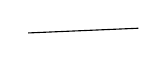
\begin{tikzpicture}
\draw (0,0) -- (1.4,0.06);
\end{tikzpicture}}

Variante de l'étude précédente pour l'extension $G_{\rho,\sigma}$ de
$\mathbb O_{12}^{*}\times H_{S_0}^{+}$ par
$\underline{M}$ (\uline{sans division par}
$\underline{\mu}_G=\{1,\omega\}_{S_0}$). Considérons d'abord la question des
scindages de la sous-extension $\underline{\mathfrak{S}}^{+}$ de
$H_{S_0}^{+}$ par $\underline{M}$ --- \unsure{elles|ils}
correspondent aux couples

\margin{113}
